\chapter{Pengenalan Pola Desain dan Pola Kreasi (Bagian 1)}

\section{Pendahuluan}

\subsection{Pengertian Pola Desain}
Pola desain (design pattern) merupakan solusi umum yang telah terbukti efektif untuk mengatasi permasalahan rekayasa perangkat lunak yang sering terjadi pada pengembangan sistem berorientasi objek. Pola-pola ini tidak berupa kode jadi, melainkan cetak biru atau template pemecahan masalah yang dapat diadaptasi ke dalam konteks spesifik proyek perangkat lunak. Pola desain muncul dari praktik terbaik yang dikumpulkan dari pengalaman para pengembang perangkat lunak dalam merancang sistem yang fleksibel, terstruktur, dan mudah dipelihara.

\subsection{Klasifikasi Pola Desain}
Pola desain umumnya diklasifikasikan ke dalam tiga kategori utama berdasarkan tujuan penggunaannya:
\begin{enumerate}
	\item \textbf{Pola Kreasi (Creational Patterns)}: Berfokus pada cara membuat objek dengan mempertimbangkan fleksibilitas dan efisiensi dalam proses instansiasi. Contohnya adalah \textit{Singleton}, \textit{Factory Method}, dan \textit{Abstract Factory}.
	\item \textbf{Pola Struktural (Structural Patterns)}: Menekankan pada cara menyusun kelas dan objek untuk membentuk struktur yang lebih besar dan fleksibel. Contohnya termasuk \textit{Adapter}, \textit{Composite}, dan \textit{Decorator}.
	\item \textbf{Pola Perilaku (Behavioral Patterns)}: Mengatur komunikasi dan tanggung jawab antar objek untuk menyederhanakan interaksi dan alur proses. Contohnya seperti \textit{Strategy}, \textit{Observer}, dan \textit{Command}.
\end{enumerate}

\subsection{Manfaat dan Tujuan Penggunaan}
Penerapan pola desain dalam pengembangan perangkat lunak membawa berbagai manfaat strategis, antara lain:
\begin{itemize}
	\item \textbf{Reusabilitas}: Pola desain memungkinkan solusi yang sama digunakan berulang kali dalam berbagai konteks dengan penyesuaian minimum.
	\item \textbf{Keterbacaan dan Komunikasi}: Pola yang telah dinamai dengan baik membantu tim pengembang memiliki pemahaman bersama tentang struktur dan tujuan desain, meningkatkan kolaborasi.
	\item \textbf{Konsistensi Arsitektural}: Dengan menggunakan pola yang terstandardisasi, arsitektur sistem menjadi lebih konsisten dan dapat diprediksi.
	\item \textbf{Pemeliharaan dan Perluasan Sistem}: Pola desain mendukung prinsip rekayasa perangkat lunak seperti \textit{Open/Closed Principle}, yang memudahkan sistem untuk diperluas tanpa mengubah struktur yang sudah ada.
\end{itemize}
Secara umum, pola desain digunakan untuk menghindari penulisan ulang solusi yang sama, mengurangi kompleksitas kode, serta meningkatkan kualitas dan umur panjang perangkat lunak yang dikembangkan.


\section{Pola Kreasi: Singleton}

\subsection{Tujuan dan Konteks Penggunaan}
Pola \textit{Singleton} adalah salah satu pola kreasi yang bertujuan untuk memastikan bahwa suatu kelas hanya memiliki satu instansi (instance) yang tersedia secara global dalam sistem. Pola ini menyediakan titik akses tunggal ke objek tersebut sehingga semua bagian program dapat menggunakannya tanpa membuat instansi baru.

Pola ini digunakan dalam situasi di mana keberadaan lebih dari satu objek dari kelas tertentu dapat menyebabkan inkonsistensi atau konflik, seperti:
\begin{itemize}
	\item Manajemen konfigurasi global
	\item Logger atau pencatatan aktivitas sistem
	\item Pengelola koneksi database
	\item Objek pengelola cache
\end{itemize}

Implementasi umum dari pola ini melibatkan penggunaan metode \texttt{static} untuk mengakses objek, serta kontrol terhadap proses instansiasi dengan menyembunyikan konstruktor kelas menggunakan \texttt{private constructor}.

\subsection{Contoh Kasus Penggunaan}
Contoh konkret penggunaan pola \textit{Singleton} dapat ditemukan pada pengembangan aplikasi yang menggunakan logger. Sebuah sistem biasanya hanya memerlukan satu objek logger untuk mencatat seluruh aktivitas, sehingga tidak efisien jika setiap bagian sistem membuat objek logger-nya sendiri.

Contoh lainnya adalah pada sistem konfigurasi, di mana data konfigurasi seperti lokasi file, alamat server, dan pengaturan jaringan hanya perlu dimuat sekali dan diakses secara global oleh seluruh komponen aplikasi.

\subsection{Kelebihan dan Kekurangan}
Pola \textit{Singleton} memiliki sejumlah kelebihan dan kekurangan yang perlu dipertimbangkan dalam perancangan perangkat lunak:

\textbf{Kelebihan:}
\begin{itemize}
	\item \textbf{Kontrol Penuh atas Instansi:} Memastikan hanya ada satu objek yang aktif selama masa hidup aplikasi.
	\item \textbf{Akses Global:} Memberikan cara mudah dan terpusat untuk mengakses instansi yang sama di seluruh sistem.
	\item \textbf{Menghemat Memori dan Sumber Daya:} Mencegah pembuatan objek yang tidak perlu secara berulang-ulang.
\end{itemize}

\textbf{Kekurangan:}
\begin{itemize}
	\item \textbf{Sulit Diuji:} Akses global dan dependensi tersembunyi membuat pengujian unit lebih kompleks, terutama jika objek \textit{Singleton} menyimpan \textit{state}. 
	\\Contoh: Jika suatu \texttt{Logger} sebagai \textit{singleton} menyimpan log terakhir sebagai state internal, maka hasil pengujian dari satu unit bisa dipengaruhi oleh hasil pengujian unit lain, karena mereka menggunakan objek logger yang sama.
	
	\item \textbf{Pelanggaran terhadap Prinsip SRP dan DIP:} Objek \textit{Singleton} sering digunakan sebagai solusi cepat yang akhirnya melanggar prinsip tanggung jawab tunggal (SRP) dan inversi dependensi (DIP).
	\\Contoh: Sebuah kelas \texttt{AppConfig} yang digunakan sebagai \textit{singleton} untuk membaca konfigurasi, tetapi kemudian juga menangani validasi dan penyimpanan ulang konfigurasi. Ini menyebabkan kelas tersebut memiliki lebih dari satu tanggung jawab (melanggar SRP), dan jika digunakan secara langsung oleh kelas lain tanpa \textit{injection}, maka bergantung pada konkret, bukan abstraksi (melanggar DIP).
	
	\item \textbf{Masalah dalam Lingkungan Multithread:} Jika tidak diimplementasikan dengan hati-hati, bisa menyebabkan kondisi balapan (\textit{race condition}) saat inisialisasi pertama kali.
	\\Contoh: Pada implementasi awal \textit{singleton} seperti:
	
	\begin{lstlisting}[style=JavaStyle]
		public class Config {
			private static Config instance;
			
			private Config() {}
			
			public static Config getInstance() {
				if (instance == null) {
					instance = new Config();
				}
				return instance;
			}
		}
	\end{lstlisting}
	
	Dua thread yang memanggil \texttt{getInstance()} secara bersamaan saat \texttt{instance} masih \texttt{null} dapat menyebabkan dua objek dibuat, yang melanggar prinsip \textit{singleton}.
\end{itemize}

\subsection{Implementasi dalam Java}

\begin{figure}[h]
	\centering
	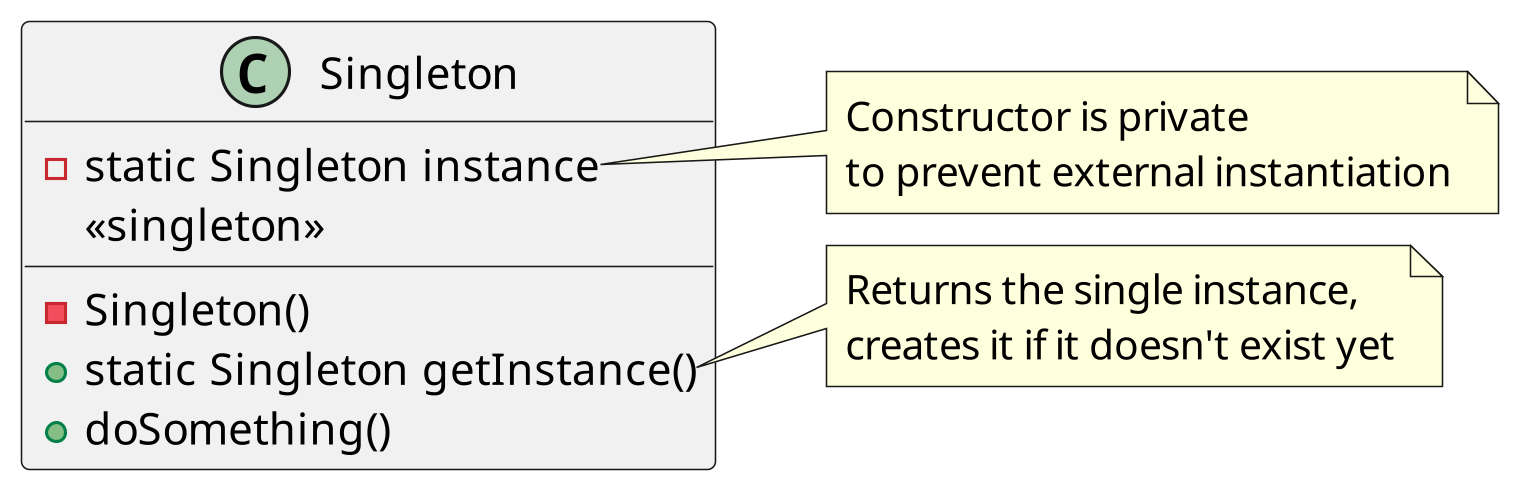
\includegraphics[width=.9\textwidth]{../figures/out/singleton.png}
	\caption{Singleton}
	\label{fig:singleton}
\end{figure}

Diagram kelas pada Gambar~\ref{fig:singleton} menggambarkan struktur dari pola Singleton. Konstruktor \texttt{Singleton()} dideklarasikan sebagai \texttt{private} untuk mencegah pembuatan objek dari luar kelas, sehingga proses instansiasi sepenuhnya dapat dikendalikan. Atribut \texttt{instance} didefinisikan sebagai \texttt{static} untuk menyimpan satu-satunya instansi dari kelas tersebut secara global. Untuk mengakses instansi ini, disediakan metode \texttt{getInstance()} yang juga bersifat \texttt{static}, memungkinkan akses global tanpa perlu melakukan instansiasi secara manual. Selain itu, kelas ini juga memiliki metode publik contoh bernama \texttt{doSomething()} yang merepresentasikan operasi umum yang dapat dilakukan oleh Singleton.


Implementasi pola \textit{Singleton} dalam Java bertujuan untuk memastikan bahwa hanya satu objek dari suatu kelas yang dapat dibuat selama siklus hidup aplikasi, dan objek tersebut dapat diakses secara global. Beberapa pendekatan dapat digunakan untuk mencapai tujuan ini, bergantung pada kebutuhan akan efisiensi, keamanan terhadap multithread, dan kemudahan implementasi.

\subsubsection*{1. Implementasi Sederhana (Tanpa Penanganan Multithread)}

Pendekatan dasar menggunakan konstruktor privat dan metode \texttt{getInstance()} statik.

\begin{lstlisting}[style=JavaStyle]
	public class SimpleSingleton {
		private static SimpleSingleton instance;
		
		private SimpleSingleton() {
			// Konstruktor privat mencegah instansiasi langsung
		}
		
		public static SimpleSingleton getInstance() {
			if (instance == null) {
				instance = new SimpleSingleton();
			}
			return instance;
		}
	}
\end{lstlisting}

Pendekatan ini sederhana namun tidak aman digunakan dalam lingkungan multithread, karena dua thread dapat membuat objek yang berbeda jika mengakses \texttt{getInstance()} secara bersamaan.

\subsubsection*{2. Singleton Aman untuk Multithread dengan Synchronized}

Untuk menghindari kondisi balapan, metode \texttt{getInstance()} dapat disinkronisasi.

\begin{lstlisting}[style=JavaStyle]
	public class ThreadSafeSingleton {
		private static ThreadSafeSingleton instance;
		
		private ThreadSafeSingleton() {}
		
		public static synchronized ThreadSafeSingleton getInstance() {
			if (instance == null) {
				instance = new ThreadSafeSingleton();
			}
			return instance;
		}
	}
\end{lstlisting}

Meskipun aman, penggunaan \texttt{synchronized} dapat memperlambat performa karena penguncian dilakukan setiap kali metode dipanggil.

\subsubsection*{3. Double-Checked Locking}

Pendekatan ini menggabungkan efisiensi dan keamanan multithread.

\begin{lstlisting}[style=JavaStyle]
	public class DoubleCheckedSingleton {
		private static volatile DoubleCheckedSingleton instance;
		
		private DoubleCheckedSingleton() {}
		
		public static DoubleCheckedSingleton getInstance() {
			if (instance == null) {
				synchronized (DoubleCheckedSingleton.class) {
					if (instance == null) {
						instance = new DoubleCheckedSingleton();
					}
				}
			}
			return instance;
		}
	}
\end{lstlisting}

Dengan menggunakan kata kunci \texttt{volatile}, Java memastikan bahwa perubahan pada variabel \texttt{instance} dapat dilihat oleh semua thread secara konsisten. Pendekatan \textit{double-checked locking} dirancang untuk meningkatkan performa dibanding metode \texttt{synchronized} penuh. Ide utamanya adalah hanya menggunakan penguncian (lock) saat instansi benar-benar belum dibuat, sehingga penguncian tidak dilakukan setiap kali \texttt{getInstance()} dipanggil. Dengan menandai variabel sebagai \texttt{volatile}, JVM tidak akan menyimpan nilai \texttt{instance} di cache thread, sehingga semua thread selalu membaca nilai terbaru dari memori utama (main memory).



\subsubsection*{4. Initialization-on-Demand Holder Idiom (Rekomendasi)}

Merupakan metode yang efisien dan thread-safe tanpa memerlukan \texttt{synchronized}.

\begin{lstlisting}[style=JavaStyle]
	public class HolderSingleton {
		private HolderSingleton() {}
		
		private static class SingletonHolder {
			private static final HolderSingleton INSTANCE = new HolderSingleton();
		}
		
		public static HolderSingleton getInstance() {
			return SingletonHolder.INSTANCE;
		}
	}
\end{lstlisting}

JVM menjamin bahwa kelas \texttt{SingletonHolder} hanya akan dimuat ketika \texttt{getInstance()} dipanggil untuk pertama kalinya, sehingga instansiasi terjadi secara malas (lazy) dan aman terhadap kondisi multithread.

Saat program dijalankan dan kelas \texttt{HolderSingleton} diakses, JVM hanya akan memuat kelas luar tersebut tanpa memuat kelas \texttt{SingletonHolder} di dalamnya. Kelas \texttt{SingletonHolder} baru akan dimuat oleh JVM ketika ada referensi langsung terhadap salah satu anggotanya, yaitu \texttt{INSTANCE}. Saat \texttt{getInstance()} dipanggil untuk pertama kali dan JVM menemukan referensi ke \texttt{SingletonHolder.INSTANCE}, barulah kelas \texttt{SingletonHolder} dimuat, dan pada saat itulah inisialisasi \texttt{private static final HolderSingleton INSTANCE = new HolderSingleton();} dieksekusi satu kali dengan jaminan thread-safe oleh JVM.


\subsubsection*{5. Menggunakan Enum (Cara Paling Aman)}

Pendekatan modern dan sangat disarankan oleh banyak pakar Java, karena enum bersifat thread-safe dan otomatis mencegah pembuatan instance tambahan.

\begin{lstlisting}[style=JavaStyle]
	public enum EnumSingleton {
		INSTANCE;
		
		public void doSomething() {
			System.out.println("Melakukan sesuatu...");
		}
	}
\end{lstlisting}

Penggunaan:
\begin{lstlisting}[style=JavaStyle]
	EnumSingleton.INSTANCE.doSomething();
\end{lstlisting}

\textbf{Catatan:} Pendekatan ini tidak cocok jika Singleton perlu mewarisi kelas lain karena enum di Java tidak dapat melakukan inheritance dari kelas biasa.

\vspace{10pt}
Dengan berbagai pendekatan di atas, pengembang dapat memilih implementasi Singleton yang sesuai berdasarkan kebutuhan sistem, kompleksitas arsitektur, dan lingkungan eksekusi yang digunakan.

\section{Pola Kreasi: Factory Method}

\subsection{Tujuan dan Konteks Penggunaan}
Pola \textit{Factory Method} merupakan salah satu pola kreasi yang digunakan untuk menghindari ketergantungan langsung terhadap kelas konkret dalam proses pembuatan objek. Tujuan utama dari pola ini adalah untuk mendefinisikan sebuah antarmuka (interface) atau kelas abstrak yang menentukan metode pembuatan objek, sementara subclass yang akan menentukan kelas konkret mana yang akan diinstansiasi.

Pola ini sangat berguna ketika:
\begin{itemize}
	\item Sistem perlu bekerja dengan objek yang tidak diketahui tipenya secara tepat di waktu kompilasi.
	\item Proses pembuatan objek melibatkan logika kompleks atau konfigurasi tertentu.
	\item Ingin menerapkan prinsip \textit{Open/Closed} dengan memungkinkan penambahan jenis objek baru tanpa mengubah kode yang sudah ada.
\end{itemize}

Factory Method sering muncul dalam kerangka kerja (framework) yang menyediakan struktur umum untuk aplikasi, sementara pengembang menyediakan implementasi spesifik dengan membuat subclass dan mengimplementasikan metode pembuatan objek.

\subsection{Contoh Kasus Penggunaan}
Salah satu contoh umum penggunaan Factory Method adalah dalam sistem GUI yang mendukung berbagai sistem operasi. Misalnya, kelas abstrak \texttt{Dialog} menyediakan metode \texttt{createButton()}, tetapi tidak menentukan secara eksplisit apakah tombol tersebut adalah \texttt{WindowsButton} atau \texttt{LinuxButton}. Subclass seperti \texttt{WindowsDialog} dan \texttt{LinuxDialog} mengimplementasikan metode \texttt{createButton()} untuk mengembalikan objek tombol yang sesuai dengan platform masing-masing.

Contoh lain adalah pada sistem pemesanan kendaraan, di mana kelas abstrak \texttt{TransportFactory} menyediakan metode \texttt{createTransport()}, dan subclass seperti \texttt{CarFactory} dan \texttt{BikeFactory} masing-masing menghasilkan objek \texttt{Car} dan \texttt{Bike} tanpa mengubah struktur kode utama.

\subsection{Kelebihan dan Kekurangan}

\textbf{Kelebihan:}
\begin{itemize}
	\item \textbf{Meningkatkan fleksibilitas dan keterluasan sistem:} Jenis objek baru dapat ditambahkan dengan membuat subclass baru tanpa mengubah kode klien.
	\item \textbf{Menerapkan prinsip SOLID:} Secara khusus mendukung prinsip Open/Closed dan Dependency Inversion dengan memisahkan pembuatan objek dari penggunaannya.
	\item \textbf{Menyederhanakan kode klien:} Kode klien tidak perlu mengetahui kelas konkret yang dibuat.
\end{itemize}

\textbf{Kekurangan:}
\begin{itemize}
	\item \textbf{Menambah kompleksitas:} Perlu membuat banyak kelas tambahan (subclass) untuk setiap jenis produk.
	\item \textbf{Sulit dibaca untuk pemula:} Struktur hirarki kelas dan pemisahan antara antarmuka dan implementasi bisa membingungkan bagi pengembang baru.
	\item \textbf{Berlebihan untuk kasus sederhana:} Jika hanya satu atau dua jenis objek yang akan dibuat, penggunaan Factory Method bisa dianggap terlalu rumit.
\end{itemize}

\subsection{Implementasi dalam Java}


\begin{figure}[h]
	\centering
	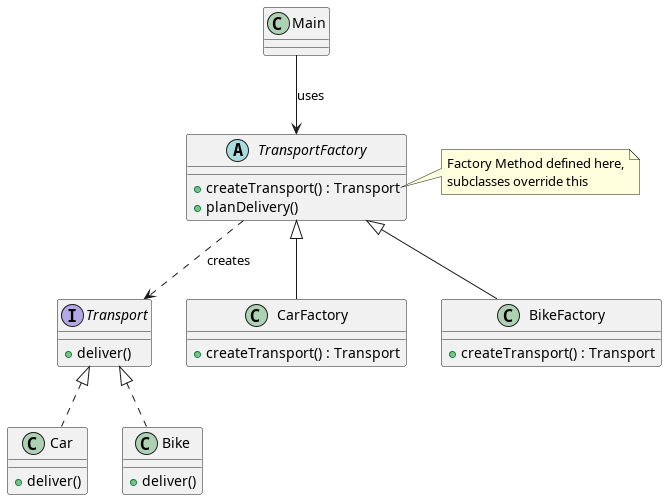
\includegraphics[width=.9\textwidth]{../figures/out/factory_method.png}
	\caption{Factory Method Pattern}
	\label{fig:factory-method}
\end{figure}


Pola \textit{Factory Method} diimplementasikan dengan mendefinisikan sebuah kelas abstrak atau antarmuka yang mendeklarasikan metode pembuatan objek, lalu subclass bertanggung jawab untuk menentukan jenis objek konkret yang akan dibuat. Hal ini memungkinkan kode klien untuk bekerja dengan antarmuka umum tanpa mengetahui detail kelas konkret yang digunakan di balik layar.

Contoh berikut menunjukkan implementasi dari sebuah sistem transportasi yang mendukung dua jenis kendaraan: mobil dan sepeda motor (Gambar \ref{fig:factory-method}).

\begin{lstlisting}[style=JavaStyle]
	// Interface produk
	public interface Transport {
		void deliver();
	}
	
	// Implementasi produk konkret
	public class Car implements Transport {
		public void deliver() {
			System.out.println("Delivery by car.");
		}
	}
	
	public class Bike implements Transport {
		public void deliver() {
			System.out.println("Delivery by bike.");
		}
	}
	
	// Kelas abstrak dengan factory method
	public abstract class TransportFactory {
		public abstract Transport createTransport();
		
		public void planDelivery() {
			Transport transport = createTransport();
			transport.deliver();
		}
	}
	
	// Implementasi factory konkret
	public class CarFactory extends TransportFactory {
		public Transport createTransport() {
			return new Car();
		}
	}
	
	public class BikeFactory extends TransportFactory {
		public Transport createTransport() {
			return new Bike();
		}
	}
	
	// Kode klien
	public class Main {
		public static void main(String[] args) {
			TransportFactory factory;
			
			factory = new CarFactory();
			factory.planDelivery(); // Output: Delivery by car.
			
			factory = new BikeFactory();
			factory.planDelivery(); // Output: Delivery by bike.
		}
	}
\end{lstlisting}

\textbf{Pembahasan:}

Implementasi di atas menggambarkan struktur dasar dari pola \textit{Factory Method}, di mana pembuatan objek didelegasikan ke subclass tanpa mengubah kode inti dari kelas utama atau klien. Kelas \texttt{TransportFactory} berfungsi sebagai kerangka dasar dengan metode abstrak \texttt{createTransport()} yang bertindak sebagai \textit{factory method}. Metode ini tidak mengembalikan objek dari kelas tertentu, tetapi dari antarmuka \texttt{Transport}, yang memungkinkan fleksibilitas dalam penggantian objek konkret.

Subclass seperti \texttt{CarFactory} dan \texttt{BikeFactory} mengimplementasikan metode \texttt{createTransport()} dan menentukan objek konkret mana yang akan dikembalikan. Dengan demikian, saat \texttt{Main} memanggil \texttt{planDelivery()}, ia tidak perlu mengetahui objek mana yang dibuat — cukup tahu bahwa objek tersebut mendukung operasi \texttt{deliver()}.

Pemisahan tanggung jawab ini mendukung prinsip \textbf{Open/Closed}, karena sistem dapat diperluas (misalnya, dengan menambahkan \texttt{TruckFactory}) tanpa mengubah kode pada kelas \texttt{TransportFactory} atau \texttt{Main}. Selain itu, penggunaan antarmuka \texttt{Transport} mendorong penerapan prinsip \textbf{Dependency Inversion}, di mana kode bergantung pada abstraksi, bukan pada implementasi konkret.

Pola ini juga sangat berguna dalam konteks framework, di mana perilaku umum didefinisikan oleh framework, tetapi pengguna dapat menyisipkan logika khusus dengan menyediakan implementasi factory method sendiri. Dengan kata lain, pola ini memungkinkan framework dan aplikasi saling berinteraksi tanpa saling bergantung secara langsung pada detail implementasi.

Dengan penerapan \textit{Factory Method}, sistem menjadi lebih modular, mudah diuji, dan lebih siap untuk menghadapi perubahan kebutuhan di masa depan. Namun demikian, penting untuk mempertimbangkan kompleksitas tambahan yang dibawa oleh hierarki kelas tambahan yang diperlukan.



\section{Pola Kreasi: Abstract Factory}

\subsection{Tujuan dan Konteks Penggunaan}

Pola \textit{Abstract Factory} merupakan pola kreasi yang bertujuan untuk menyediakan antarmuka (interface) untuk membuat keluarga objek-objek terkait (related) atau tergantung satu sama lain tanpa harus menyebutkan kelas konkret mereka secara langsung. Dengan kata lain, pola ini digunakan ketika sistem perlu membuat sekumpulan objek yang harus digunakan secara bersama-sama dan kompatibel, namun tidak ingin mengikat implementasi terhadap kelas konkret secara langsung.

Pola ini sering digunakan dalam konteks di mana:
\begin{itemize}
	\item Sistem harus bekerja dengan berbagai varian atau konfigurasi dari objek-objek yang saling terkait.
	\item Proses pembuatan objek kompleks melibatkan hierarki kelas dan dependensi antarobjek.
	\item Dibutuhkan mekanisme untuk mengganti keluarga produk dengan mudah tanpa mengubah kode program utama.
\end{itemize}

Abstract Factory sering dianggap sebagai “factory dari factory” karena ia menciptakan objek-objek factory (pembuat) lain yang masing-masing bertanggung jawab atas pembuatan objek dalam satu keluarga.

\subsection{Contoh Kasus Penggunaan}

Salah satu contoh klasik dari penggunaan \textit{Abstract Factory} adalah dalam pengembangan antarmuka pengguna (GUI) yang mendukung berbagai sistem operasi atau tema (look and feel). Misalnya, aplikasi desktop yang harus mendukung tampilan untuk sistem Windows dan macOS. Dalam hal ini, terdapat dua keluarga produk: \texttt{Button} dan \texttt{Checkbox}. Abstract Factory digunakan untuk menciptakan \texttt{WinButton} dan \texttt{WinCheckbox} untuk Windows, serta \texttt{MacButton} dan \texttt{MacCheckbox} untuk macOS, tanpa mengubah kode program utama.

Contoh lain adalah sistem database yang harus mendukung berbagai vendor seperti MySQL, PostgreSQL, atau Oracle. Setiap vendor membutuhkan serangkaian objek berbeda untuk koneksi, query builder, dan migrasi. Dengan \textit{Abstract Factory}, sistem dapat menyediakan \texttt{MySQLFactory}, \texttt{PostgresFactory}, dan \texttt{OracleFactory}, masing-masing menciptakan produk-produk yang sesuai tanpa perlu mengubah kode klien.

\subsection{Kelebihan dan Kekurangan}

\textbf{Kelebihan:}
\textbf{Kelebihan:}
\begin{itemize}
	\item \textbf{Konsistensi antar produk:} Semua objek yang dibuat oleh satu keluarga factory saling kompatibel dan sesuai digunakan bersama. \\
	\textit{Contoh:} \texttt{WinFactory} menghasilkan \texttt{WinButton} dan \texttt{WinCheckbox} yang didesain dengan gaya antarmuka pengguna Windows. Dengan menggunakan satu factory, tampilan dan perilaku seluruh elemen UI menjadi konsisten sesuai tema.
	
	\item \textbf{Mendukung prinsip SOLID:} Khususnya prinsip \textbf{Dependency Inversion} dan \textbf{Open/Closed}, karena kode klien bergantung pada abstraksi dan mudah diperluas untuk menambahkan keluarga produk baru. \\
	\textit{Contoh:} Kelas \texttt{Application} hanya bergantung pada \texttt{GUIFactory} dan antarmuka produk seperti \texttt{Button} dan \texttt{Checkbox}. Jika ditambahkan \texttt{LinuxFactory}, kode \texttt{Application} tidak perlu diubah sama sekali.
	
	\item \textbf{Isolasi dari kelas konkret:} Klien tidak mengetahui dan tidak bergantung pada implementasi produk secara langsung. \\
	\textit{Contoh:} Klien cukup memanggil \texttt{factory.createButton()} tanpa harus tahu apakah yang dihasilkan adalah \texttt{MacButton} atau \texttt{WinButton}. Hal ini memungkinkan kode lebih modular dan mudah diuji dengan substitusi implementasi.
	
	\item \textbf{Mempermudah penggantian konfigurasi:} Cukup dengan mengganti implementasi factory, seluruh komposisi sistem bisa berubah (misalnya, dari tampilan tema terang ke tema gelap). \\
	\textit{Contoh:} Dalam aplikasi grafis, jika pengguna memilih "Dark Theme", sistem tinggal menginstansiasi \texttt{DarkThemeFactory} sebagai \texttt{GUIFactory}, tanpa harus mengganti logika tampilan di bagian lain program.
\end{itemize}

\textbf{Kekurangan:}
\begin{itemize}
	\item \textbf{Kompleksitas struktur kelas:} Membutuhkan banyak antarmuka dan kelas untuk setiap keluarga produk. \\
	\textit{Contoh:} Untuk dua jenis produk (misalnya \texttt{Button} dan \texttt{Checkbox}) dan tiga varian (Windows, Mac, Linux), diperlukan minimal 3 factory, 6 kelas produk konkret, dan 2 antarmuka produk.
	
	\item \textbf{Kurang fleksibel untuk produk yang berdiri sendiri:} Jika hanya satu atau dua produk yang perlu diganti, Abstract Factory bisa terasa terlalu berlebihan dibanding Factory Method biasa. \\
	\textit{Contoh:} Jika aplikasi hanya ingin mengganti implementasi \texttt{Button} saja berdasarkan konfigurasi, menggunakan Abstract Factory untuk seluruh UI akan menghasilkan struktur yang tidak proporsional dan membingungkan.
	
	\item \textbf{Tingkat abstraksi tinggi:} Membingungkan bagi pemula karena melibatkan kombinasi berbagai pola seperti Interface, Factory Method, dan Composition. \\
	\textit{Contoh:} Seorang pengembang baru mungkin kesulitan memahami relasi antara \texttt{GUIFactory}, produk abstrak (\texttt{Button}, \texttt{Checkbox}), dan implementasi konkrit, karena semua objek diciptakan secara tidak langsung.
\end{itemize}


\subsection{Implementasi dalam Java}

Pola \textit{Abstract Factory} diimplementasikan dalam Java dengan mendefinisikan sekumpulan antarmuka produk dan sebuah antarmuka pabrik (\texttt{Factory}) yang bertanggung jawab atas pembuatan produk-produk tersebut. Implementasi konkret dari pabrik akan menciptakan produk-produk yang sesuai dengan satu keluarga atau varian tertentu.

Contoh berikut menunjukkan sistem GUI yang dapat menghasilkan dua keluarga produk: \texttt{Button} dan \texttt{Checkbox}, masing-masing dengan implementasi untuk platform Windows dan macOS (Gambar \ref{fig:factory-abstract})).

\begin{figure}[h]
	\centering
	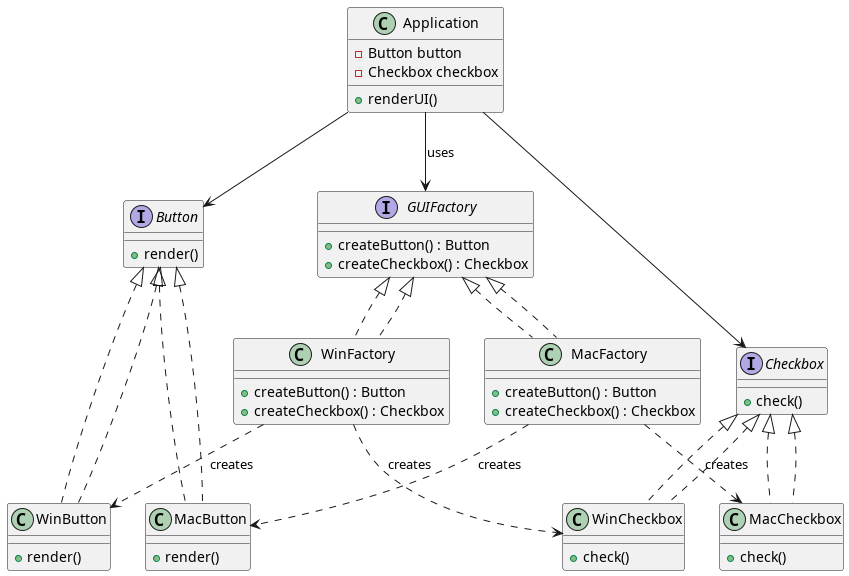
\includegraphics[width=.9\textwidth]{../figures/out/factory_abstract.png}
	\caption{Factory Method Pattern}
	\label{fig:factory-abstract}
\end{figure}

\begin{lstlisting}[style=JavaStyle]
	// Produk 1: Button
	public interface Button {
		void render();
	}
	
	public class WinButton implements Button {
		public void render() {
			System.out.println("Render Windows-style button.");
		}
	}
	
	public class MacButton implements Button {
		public void render() {
			System.out.println("Render macOS-style button.");
		}
	}
	
	// Produk 2: Checkbox
	public interface Checkbox {
		void check();
	}
	
	public class WinCheckbox implements Checkbox {
		public void check() {
			System.out.println("Check Windows-style checkbox.");
		}
	}
	
	public class MacCheckbox implements Checkbox {
		public void check() {
			System.out.println("Check macOS-style checkbox.");
		}
	}
	
	// Abstract Factory
	public interface GUIFactory {
		Button createButton();
		Checkbox createCheckbox();
	}
	
	// Concrete Factory: Windows
	public class WinFactory implements GUIFactory {
		public Button createButton() {
			return new WinButton();
		}
		
		public Checkbox createCheckbox() {
			return new WinCheckbox();
		}
	}
	
	// Concrete Factory: macOS
	public class MacFactory implements GUIFactory {
		public Button createButton() {
			return new MacButton();
		}
		
		public Checkbox createCheckbox() {
			return new MacCheckbox();
		}
	}
	
	// Client code
	public class Application {
		private Button button;
		private Checkbox checkbox;
		
		public Application(GUIFactory factory) {
			button = factory.createButton();
			checkbox = factory.createCheckbox();
		}
		
		public void renderUI() {
			button.render();
			checkbox.check();
		}
		
		public static void main(String[] args) {
			GUIFactory factory;
			
			// Bisa diganti dengan konfigurasi eksternal
			factory = new WinFactory();
			Application app1 = new Application(factory);
			app1.renderUI();
			
			factory = new MacFactory();
			Application app2 = new Application(factory);
			app2.renderUI();
		}
	}
\end{lstlisting}

\textbf{Pembahasan:}

Kode di atas memperlihatkan struktur khas dari pola \textit{Abstract Factory}, di mana terdapat dua jenis produk: \texttt{Button} dan \texttt{Checkbox}. Masing-masing memiliki dua implementasi: satu untuk Windows dan satu untuk macOS.

Antarmuka \texttt{GUIFactory} mendefinisikan kontrak pembuatan kedua jenis produk. \texttt{WinFactory} dan \texttt{MacFactory} adalah implementasi konkret yang membuat objek produk sesuai dengan gaya sistem operasi masing-masing. Kode klien dalam kelas \texttt{Application} tidak perlu mengetahui kelas konkret apa yang digunakan. Ia cukup bergantung pada \texttt{GUIFactory}, dan akan mendapatkan objek-objek yang konsisten sesuai konfigurasi.

Pola ini memungkinkan sistem untuk dengan mudah berganti tema atau platform tanpa memodifikasi logika aplikasi. Cukup dengan mengganti implementasi \texttt{GUIFactory}, seluruh UI dapat disesuaikan dengan lingkungan yang diinginkan. Pendekatan ini mendorong pengembangan sistem yang fleksibel, modular, dan mudah diuji, terutama saat mengelola variasi produk dalam jumlah besar.

\section{Perbandingan Factory Method dan Abstract Factory}

\subsection{Penjelasan Konseptual}

\textbf{Factory Method} adalah pola kreasi yang bertujuan untuk menyediakan mekanisme pembuatan objek tunggal dengan menunda pemilihan kelas konkret ke subclass. Struktur umum dari pola ini melibatkan satu metode factory, seperti \texttt{createProduct()}, yang di-override oleh subclass untuk mengembalikan produk konkret. Fokus utamanya adalah pada fleksibilitas dan perluasan, dengan memberi subclass tanggung jawab menentukan implementasi yang sesuai.\\
\textit{Contoh:} Dalam sistem transportasi, terdapat antarmuka \texttt{TransportFactory} dengan metode \texttt{createTransport()}. Subclass seperti \texttt{CarFactory} dan \texttt{BikeFactory} akan masing-masing mengembalikan objek \texttt{Car} dan \texttt{Bike}.

\textbf{Abstract Factory}, di sisi lain, berfungsi untuk menyediakan antarmuka dalam menciptakan \textit{keluarga produk terkait} yang dirancang untuk digunakan bersama secara konsisten. Pola ini mengelompokkan beberapa metode factory dalam satu antarmuka, seperti \texttt{createButton()} dan \texttt{createCheckbox()}, dengan setiap concrete factory bertugas mengimplementasikan seluruh metode tersebut secara seragam. Fokus dari pola ini adalah pada konsistensi konfigurasi dan kompatibilitas antar objek dalam satu keluarga.\\
\textit{Contoh:} \texttt{GUIFactory} mendefinisikan metode \texttt{createButton()} dan \texttt{createCheckbox()}. \texttt{WinFactory} dan \texttt{MacFactory} akan menghasilkan elemen UI yang sesuai dengan gaya Windows atau macOS secara konsisten. 


\begin{table}
	\centering
	\begin{tabular}{|p{0.16\textwidth}|p{0.28\textwidth}|p{0.45\textwidth}|}
		\hline
		\rowcolor{gray!20} 
		\textbf{Aspek} & \textbf{Factory Method} & \textbf{Abstract Factory} \\
		\hline
		Tujuan & Menentukan objek konkret dalam subclass & Membuat keluarga produk yang kompatibel \\
		\hline
		Jenis produk & Satu jenis produk & Beberapa jenis produk dalam satu keluarga \\
		\hline
		Struktur & Satu metode factory & Beberapa metode factory dalam satu antarmuka \\
		\hline
		Jumlah kelas produk & Biasanya tunggal & Beberapa (kompleksitas lebih tinggi) \\
		\hline
		Polimorfisme produk & Produk dari satu hierarki & Produk dari beberapa hierarki \\
		\hline
		Ketergantungan & Klien bergantung pada satu produk abstrak & Klien bergantung pada beberapa produk abstrak \\
		\hline
		Contoh umum & \texttt{createTransport()} & \texttt{createButton()}, \texttt{createCheckbox()} \\
		\hline
		Kompleksitas & Lebih sederhana & Lebih kompleks \\
		\hline
	\end{tabular}
	\caption{Perbandingan Factory Method dan Abstract Factory}
	\label{tab:factory-comparison}
\end{table}


\subsection{Kapan Menggunakan?}

Lihat Tabel \ref{tab:factory-comparison} untuk perbandingan. Pola \textbf{Factory Method} sebaiknya digunakan ketika hanya perlu membuat satu jenis objek, khususnya jika sistem membutuhkan fleksibilitas untuk memilih implementasi produk di tingkat subclass. Pola ini juga cocok apabila proses instansiasi perlu ditunda atau dikontrol berdasarkan kondisi tertentu.

Sebaliknya, pola \textbf{Abstract Factory} lebih tepat digunakan ketika sistem memerlukan beberapa objek yang saling terkait dan harus digunakan bersama, seperti komponen UI dalam satu tema tampilan. Pola ini sangat bermanfaat jika seluruh konfigurasi produk perlu diganti secara menyeluruh, seperti saat berpindah dari tema terang ke tema gelap, atau dari platform Windows ke macOS, serta saat menjaga konsistensi antar produk menjadi prioritas utama. 


\section{Penutup}

Pola desain merupakan fondasi penting dalam pengembangan perangkat lunak berorientasi objek yang bersifat modular, terstruktur, dan mudah dikembangkan. Dalam bab ini, telah dibahas tiga pola kreasi utama—\textit{Singleton}, \textit{Factory Method}, dan \textit{Abstract Factory}—yang masing-masing menawarkan pendekatan berbeda dalam mengelola proses pembuatan objek. Pola \textit{Singleton} memastikan hanya ada satu instansi dalam sistem, \textit{Factory Method} memberikan fleksibilitas dalam memilih jenis objek di tingkat subclass, sedangkan \textit{Abstract Factory} memungkinkan penciptaan keluarga objek yang saling terkait dan konsisten.

Pemahaman dan penerapan ketiga pola ini tidak hanya membantu pengembang dalam mengelola kompleksitas sistem, tetapi juga memperkuat prinsip-prinsip desain perangkat lunak seperti enkapsulasi, inversi dependensi, dan keterbukaan terhadap perluasan. Pemilihan pola yang tepat sebaiknya disesuaikan dengan konteks dan kebutuhan arsitektur aplikasi, serta mempertimbangkan tingkat skalabilitas dan konsistensi antar komponen sistem yang ingin dicapai.
